%\documentclass[preprint,notitlepage]{revtex4-1}
\documentclass[prl,twocolumn,notitlepage]{revtex4-1}
\usepackage{graphicx}
\usepackage{epstopdf}
\usepackage{amsmath}
\usepackage{hyperref}
\usepackage{booktabs}
\usepackage{color}

\usepackage{SIunits}
\newcommand{\wstar}{-0.023}
\newcommand{\Qstar}{0.25}

\setlength{\tabcolsep}{10pt}

\newenvironment{sistema}%
  {\left\lbrace\begin{array}{@{}l@{}}}%
  {\end{array}\right.}

\usepackage{xr}
\externaldocument[M-]{glass}

\usepackage{hyperref}

%% HACKS %%
 
% For section headers starting with S
\renewcommand{\thesection}{S.\arabic{section}}
\renewcommand{\thesubsection}{\thesection.\arabic{subsection}}
 
% Hack for making SOM Equations Conform to Science Format
%
% e.g. (S1), (S2), etc
% Requires AMS
\makeatletter %% With ams
\def\tagform@#1{\maketag@@@{(S\ignorespaces#1\unskip\@@italiccorr)}}
\makeatother
 
% Hack for making figures Say \figurename S\thefigure, e.g. Figure S1:
\makeatletter
\makeatletter \renewcommand{\fnum@figure}
{\textbf{Supplementary~Figure~S\thefigure}}
\makeatother
 
% use bibnumfmt to change style at the end of the document
%\renewcommand{\bibnumfmt}[1]{[S#1]}
% citenumfont command adds S to all numbers
%\renewcommand{\citenumfont}[1]{\textit{S#1}}
 
%\renewcommand{\figurename}{Figure}
 
 
 
%END HACKS

\begin{document}
\title{SUPPLEMENTARY INFORMATION for ``Roles of icosahedral and crystal-like order \\ in hard spheres glass transition''} 
%\title{Role of structural heterogeneity of the supercooled liquid\\ in the crystallization of hard spheres}
%\title{On the origin of polymorphism during the nucleation of hard spheres}
%\title{On the origin of crystal polymorphism in hard spheres}
%\title{Selection principle of polymorphs upon crystallization \\ in hard spheres}
%\title{Role of orientational order in the crystallization of hard spheres}
%\title{On the microscopic mechanism of crystallization in hard spheres:\\ role of bond
%orientational ordering}
%\title{Crystal Polymorphism starts before crystallization}
%\title{Crystal Polymorphism starts before crystallization}
%\title{Crystal Polymorphism before crystallization}


\author{Mathieu Leocmach} 

\author{Hajime Tanaka}
\email{tanaka@iis.u-tokyo.ac.jp}
\affiliation{ {Institute of Industrial Science, University of Tokyo, 4-6-1 Komaba, Meguro-ku, Tokyo 153-8505, Japan} }

%\date{}

\maketitle

\section*{Particle localisation and sizing}

Particle-level confocal microscopy experiments usually access the coordinates of the particles via the algorithm proposed by \citet{Crocker1996}. The original noisy image is blurred by convolution with a Gaussian kernel of width $\sigma$ to yield a soft peak per particle. Local intensity maxima within this blurred image give the coordinates of the particles with pixel resolution. Sub-pixel resolution ($0.1\sim0.3$~pixels error) can be achieved by taking the centre of mass of a neighbourhood around the local maxima. The extension of this algorithm in 3D has been done in two ways: either tracking particles in each confocal plane and reconstructing the results (2D-flavour)~\citep{dinsmore2001tdc}, or full image analysis on three dimensional pictures (3D-flavour)~\citep{vanblaaderen1995rss, Lu2007}.

The choice of the width $\sigma$ of the blurring kernel is critical: if it is too small, then the intensity profile is flat near the centre  of a particle, leading to multiple and ill-localized maxima per particle; if it is too large, then the peaks of nearby particles overlap, leading to shifts in the detected positions, or even fusion of the particles (only one particle detected instead of two). If the colloids are fairly monodisperse one can argue (at least in the 3D-flavour) that there exists a range of possible width where the choice of $\sigma$ has almost no effect on the number of particles detected. Choosing $\sigma$ within this range gives confidence in the localisation results.

\begin{figure*}
\begin{center}
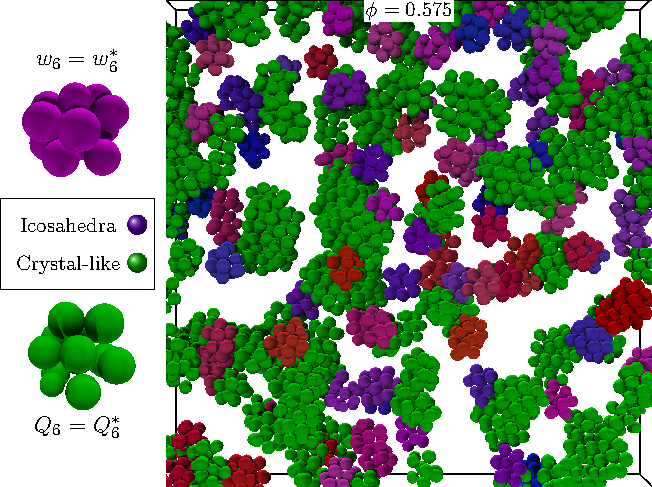
\includegraphics{generate_figures-figure5.pdf}
\end{center}
\caption{\textbf{Visualisation of the results of various tracking methods for the same portion of image.} The circles on each picture are identical and result from 2D multiscale tracking of each XY slice of the 3D pictures. \textbf{a,} XZ and YZ slices of the image (fake colors). \textbf{b,} Multiscale 3D tracking. Spheres are drawn with the radius determined by the tracking methods. \textbf{c-h,} Crocker and Grier in 3D with blurring radius increasing from \unit{2}{px} to \unit{4.5}{px} by steps of \unit{0.5}{px} (Sphere radii correspond to the blurring radius).}
	\label{fig:localise}
\end{figure*}
\begin{figure*}
\begin{center}
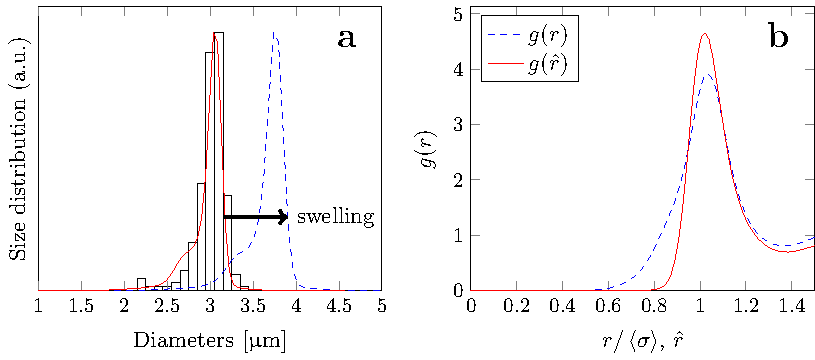
\includegraphics{generate_figures-figure6.pdf}
\end{center}
	\caption{\textbf{Sizing of our colloids.} \textbf{a,b,} XY and XZ slices (detail) of a typical confocal 3D image of our sample. Note the excellent Z resolution, almost not affected by the point spread function. \textbf{c,} Size distribution estimated \emph{in situ} (dashed line) by our multiscale algorithm ($\sim 1.7\times 10^6$ instantaneous sizing). Comparison with the size distribution estimated from \textsc{sem} of only $140$ dry particles (steps) is possible once $23\%$ of swelling of particle diameters is taken into account (full line). \textbf{d,} First peak of the radial distribution function with (full line) and without (dashed) the individual sizes data. Taking into account the measured sizes rectifies the effect of the polydispersity: the peak is thinner and higher.}
	\label{fig:sizing}
\end{figure*}

However, we found that no such ``good blur width'' exists in our polydisperse sample (see Supplementary Fig.~S\ref{fig:localise}c-h). The detection of smaller particles with small blurring widths leads to the failure in detecting properly the larger particles. This unacceptable failure of the \citet{Crocker1996} algorithm, as well as the want of the particles' radii data, triggered our design of a novel localisation algorithm that would be robust even for a system of finite polydispersity, which is unavoidable in real experiments. Here we briefly disclose our method, leaving full details to a future publication.

The key notion to detect objects of unknown and possibly diverse sizes in an image is the \emph{scale space}~\cite{Lindeberg1993}. A popular implementation for isotropic objects (or ``blobs'') is the Scale Invariant Feature Transform (\textsc{sift}) of \citet{Lowe2004}. It consists  in blurring the image by Gaussian kernels of logarithmically increasing widths ($\sigma_{i+1} = 2^{1/n} \sigma_i$, with $n$ a fixed integer, $n=3$ being a good choice) and taking the difference between consecutive blurred images. The difference of Gaussians (DoG) response function defined in this way depends on the position in space and on the scale. Bright objects in the original image are detected as local minima of the DoG in both space and scale, thus localisation and \emph{size} are determined simultaneously, without any assumption on the target size (see Supplementary Fig.~S\ref{fig:localise}b).

The \textsc{sift} is often used to match between different images from complex objects consisting of many rigidly linked blobs and further characterised by local histograms~\citep{Lowe2004}. To our knowledge, this method was never used for the quantitative localisation and sizing of independent single-blob objects like spherical colloids. The object-by-object optimal scale determination allows us to perform the spatial sub-pixel resolution step for each object on an image that is blurred just enough to have neither a flat intensity profile nor a nearby peak overlap. This leads to a spatial resolution below $0.3$~pixels when two $10$-pixels wide particles are at hard-core contact, and less than $0.03$~pixels error ($0.3\%$ of the diameter) when any other particle's surface is further than $1$~pixel from the surface of the particle of interest.

At infinite dilution the optimal scale $\sigma^*$ is simply proportional to the radius $R$ of the particle. Assuming a binary ball object, one finds\textcolor{blue}{
\begin{equation}
	R = \sigma^* \sqrt{\frac{6\ln \alpha}{1-\alpha^{-2}}}, 
	\label{eq:scale_dil}
\end{equation}
where $\alpha = 2^{1/n}$ is the step of the discrete scale space. Eq.~(S\ref{eq:scale_dil}) allows to translate the $n$-dependent $\sigma^*$ to the parameter-free real radius of the particle.} The error on $R$ does depend on the number of subdivisions.

We found that the radius of an isolated pixelated ball can be indeed measured within $0.3\%$ relative error with this method, provided a sub-scale resolution step similar to the spatial sub-pixel resolution step. The point spread function of real confocal images acts like an blur in the Z direction. As long as this blur can be approximated to a Gaussian, one can show that it affects the proportionality constant without adding a constant term in Eq.~(S\ref{eq:scale_dil}).

In dense suspensions, the neighbouring particles influence the scale dependence of DoG response. This effectively shifts the minima of the DoG towards smaller scales, leading to smaller radii if one uses Eq.~(S\ref{eq:scale_dil}) alone. Assuming once again binary ball objects, one can take this coupling into account and construct an $N\times N$ system, with $N$ the number of particles, whose solutions are the radii and whose coefficients depend on the inter-particle distances. This system is actually very sparse (less than two dozen non-zero coefficients per line, even in the dense suspensions studied here) and the results converge in about two iterations. In synthetic images we measured the error in the resulting radii to be around $1\%$. In an experimental image, the particles are not uniformly bright due to synthesis imperfection (quantity of dye fixed by each particle) and photo bleaching. If one does not take into account the relative brightness of the particles the less bright will appear smaller. We were able to relate the magnitude of the DoG response (environment-dependent) to a measure of the brightness and thus correct the influence of the relative brightness on the sizing.

Supplementary Figure~S\ref{fig:sizing}c shows the size distribution of the suspensions investigated in the main text. Once a solvent swelling of $23\%$ in radius is taken into account, our \emph{in situ} measurements compare very well with the size distribution obtained from scanning electron microscopy (\textsc{sem}) of the same `dry' colloids. The polydispersity measured \emph{in situ} is $6.9\%$, where the polydispersity computed from \textsc{sem} is $6.2\%$.

The consistency of our method can be checked by constructing the radial distribution function $g(r)$. In monodisperse hard spheres, the $g(r)$ has a sharp first peak at $r=2R$ corresponding to hard core contact. Polydispersity implies hard core contacts at various $r$ and thus broadens the peak. One can recover a sharp peak by constructing $g(\hat{r})$, with $\hat{r}_{ij} = r_{ij}/(R_i+R_j)$. In Supplementary Fig.~S\ref{fig:sizing}d we successfully used the sizes measured by our method to rectify the first peak.

Recently \citet{Kurita2011,Kurita2011b} have designed a sizing method using particle coordinates from confocal experiments. However their method do not work at the image processing level and relies on coordinates extracted via the \citet{Crocker1996} algorithm which, as described above, is defective when the size distribution is too broad. It may be possible to combine the two methods by feeding our coordinates and size as input to their method. We would expect an increase in sizing precision when the particles are close to contact.


\section*{Difference between {\sc mrco} and crystal nuclei}

\begin{figure}
\begin{center}
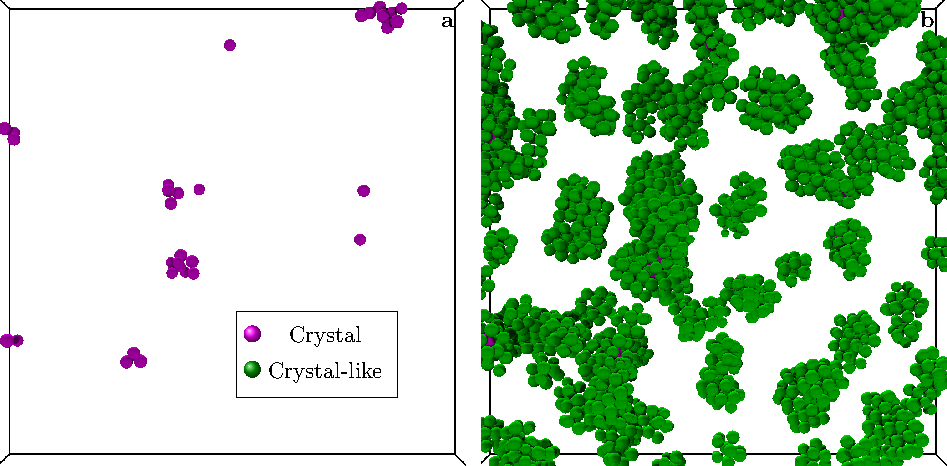
\includegraphics{generate_figures-figure4.pdf}
\end{center}
\caption{\textbf{Medium-range bond orientational order and crystalline bonds} {\bf a,} Particles with more than $7$ crystalline bonds.  {\bf b,} Particles with $Q_6>Q_6^*$ and their neighbours are also plotted for comparison. Crystalline particles are always included in high $Q_6$ regions and thus a part of bond order parameter fluctuations. They do not grow and thus appear only transiently.}
	\label{fig:X_3D}
\end{figure}

To avoid any confusion between our imperfect crystal-like order and well-formed but small transient crystals, we detect crystal nuclei \emph{via} the most standard method in the literature~\cite{ReintenWolde1996, Zaccarelli2009}. For each neighbouring particle, we compute the normalized scalar product of the (non coarse-grained) $q_{6 m}$:
\begin{equation}
	s(i,j) = \frac{
		\sum_{m=-6}^{6} q_{6 m}(i) q_{6 m}^{*}(j)
	}{
		\sqrt{\sum_{m=-6}^{6} |q_{6 m}(i)|^2} \sqrt{\sum_{m=-6}^{6} |q_{6 m}(j)|^2}
	}.
	\label{eq:boo_dot_product}
\end{equation}
The bond between particles $i$ and $j$ is considered crystalline if $s_{ij}>0.7$~\cite{Zaccarelli2009}. A particle is crystalline if more than half of its bonds ($\geq 7$) are crystalline. 

The polydispersity is an important controlling factor which determines the ease of crystallization of colloidal suspensions (see, e.g., \cite{Zaccarelli2009}). 
The polydispersity of our sample was high enough to prevent crystallisation in bulk over our experimental timescales. 
However, heterogeneous nucleation from the walls sometimes interfered our experiments, thus we had to discard such samples that accompanied crystallisation. 
We find no large crystal nucleus in our samples analysed in the text. Even at deep supercooling a crystal nucleus never gathers more than 8 particles, and in total truly crystalline particles account for less than $1\%$ of the system. We emphasize that the size of these crystals is still smaller than the critical nucleus size (between 2 and 3 particle diameters according to~\cite{Auer2001} and classical nucleation theory). This was confirmed by the fact that crystal-like solid regions (see Supplementary Fig.~S\ref{fig:X_3D}a) appear only transiently without growth. In other words, we never observed crystal nucleation in bulk for our samples. Supplementary Figure~S\ref{fig:X_3D} compares the spatial extent of crystal nuclei with that of the crystal-like clusters. Visual inspection of the patterns in Fig.~\ref{M-fig:3D}e and Supplementary Fig.~S\ref{fig:X_3D}a,b  demonstrates that trivial crystallisation can be responsible for neither the spatial extent of the dynamical heterogeneities nor glassy slow dynamics.

However, sub-critical nuclei are not unrelated to crystal-like order. Nuclei are systematically embedded into much larger \textsc{mrco}. One can explain this phenomenon as perfect wetting of the nuclei by coherently bond-ordered regions. However, examples of crystal-like structures without an embedded crystal nucleus, in addition to the continuity of $Q_6$ values (Fig.~\ref{M-fig:maps}), rather suggests that the crystal nuclei are the extreme part of the bond order fluctuations. Indeed it has been shown in hard spheres~\cite{OMalley2005, Schilling2010, Kawasaki2010c, Russo2011}, gaussian-core model~\cite{Russo2012} and probably Wahnstr\"om binary Lennard-Jones~\cite{Pedersen2010} that parts of \textsc{mrco}, fluid regions with a structure reminiscent of the crystal, act as precursors to crystallisation if the local density there is high enough. However in these systems the presence of precursors to crystallisation does not imply the formation of a critical nucleus and growth. Furthermore, \textsc{mrco} is always present (transiently) in the supercooled liquid and its size is often used to characterise dynamical heterogeneity of the supercooled liquid: \textsc{mrco} are usual fluctuations of the system, as common as the fast and slow regions of the dynamic heterogeneity~\cite{tanaka2010critical}. We also note that the average density within \textsc{mrco} is the same as within disordered liquid regions and thus different from within crystal nuclei~\cite{Kawasaki2010c}.

\section*{Dynamics}

\begin{figure}
\begin{center}
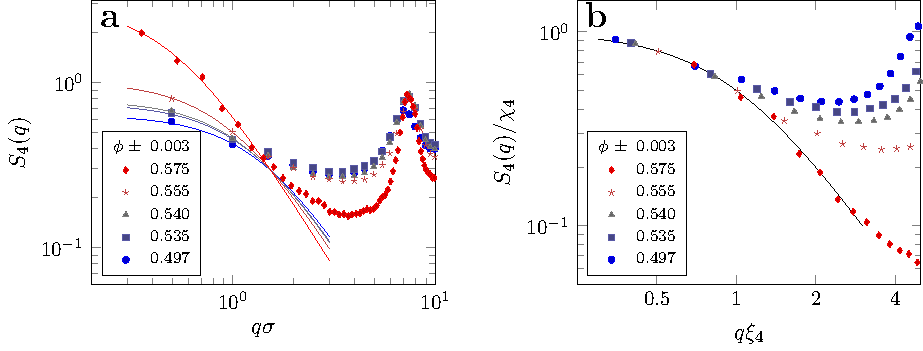
\includegraphics{generate_figures-figure8.pdf}
\end{center}
\caption{\textbf{Four-point structure factor} at different volume fractions, computed for a time difference $t$ so that $\chi_4(t)$ is maximum.}
	\label{fig:S4}
\end{figure}

To define the characteristic length scale of the dynamic heterogeneity, we define a microscopic overlap function $w_n(t)$ so that $w_n(t)=1$ if the particle $n$ moved less than $0.3\langle\sigma\rangle$ during $t$ and $w_n(t)=0$ otherwise. From this we can compute the four-point structure factor~\cite{Flenner2011}
\begin{equation}
	S_4(q,t) = N^{-1}(\left\langle W(\vec{q},t) W(-\vec{q},t) \right\rangle - | \left\langle W(\vec{q},t) \right\rangle^2 |)
	\label{eq:S4}
\end{equation}
where $W(\vec{q},t)$ is the Fourier transform of $w_n(t)$
\begin{equation}
	W(\vec{q},t) = \sum_n w_n(t)\exp(-\imath \vec{q}\cdot\vec{r}_n(0))
\end{equation}

To give a more understandable picture, we note that $S_4(q,t)$ is the structure factor of a system containing only the ``slow'' (overlapping) particles divided by the ratio of overlapping particles. Our experimental data do \emph{not} have periodic boundary conditions, so we must use a window function to ensure the correct correlation, especially at small $q$. Here we use Hamming window, but we checked that our results are not affected by other reasonable choices of window function. Results are shown in Supplementary Fig.~S\ref{fig:S4}.

The long wavelength (small wave-vector) behaviour of $S_4(q,t)$ is well described by the asymptotic Ornstein-Zernike in Fourier space:
\begin{equation}
	S_4(q,t) \approx \frac{\chi_4(t)}{1+\xi_4(t)^2 q^2} \quad \text{as } q\rightarrow 0
	\label{eq:OZ_Fourier}
\end{equation}
where $\chi_4(t)$ is the four-point susceptibility and $\xi_4(t)$ is the four-point correlation length, both depending on the time difference $t$. We found that at each volume fraction the maximum of $\chi_4(t)$ is reached at times longer that the relaxation time $\tau_\alpha$. In summary, we have
\begin{equation}
t^{dh} \leq \tau_\alpha \leq t_{\chi_4}.
\end{equation}
For clarity, we omit time dependence in $S_4$, $\xi_4$ and $\chi_4$ when $t=t_{\chi_4}$.

In Supplementary Fig.~S\ref{fig:S4} we show the fit by Eq.~(\ref{eq:OZ_Fourier}) of $S_4(q)$. \textcolor{blue}{As stressed in \citep{Flenner2011}, the value $S_4(q\rightarrow 0)$ is crucial for the quality of the fit. In the thermodynamic limit we have
\begin{equation}
\chi_4 = (\langle N_s^2\rangle - \langle N_s\rangle^2) /  \langle N\rangle,
\end{equation}
where $N$ is the total number of particles and $N_s$ is the number of overlapping particles. In a simulation with a fixed $N$ and a limited size, some fluctuations are forbidden, thus the above equation do not give the right value of $\chi_4$ (see \citep{Flenner2011}). However in our experiments we are looking at a small portion of a very large system (the whole colloidal suspension), thus we can use time average to sample all the fluctuations of this large system, and the above equation becomes exact. We use this value as $S_4(q=0)$ in our fitting procedure.} 

The volume fraction dependence of the resulting correlation length is plotted in the inset of Fig.~\ref{M-fig:vft} of the main text. The dynamical correlation length $\xi_4$ almost coincides with the static one $\xi_6$, which further supports a static structural origin of dynamic heterogeneity in our system. \textcolor{blue}{We do not claim universality on the absolute value of both correlation lengths; indeed our $\xi_4$ is shorter than the one of \citet{Flenner2011} at the same distance to $\phi_0$. This may be linked to the difference in fragility between the two systems (or their underlying crystal).}

As an aside, we have also computed the mobility-mobility spatial correlation function~\cite{Donati1999}
\begin{equation}
	\mathcal{G}_u(r,t) = \frac{
		\left\langle \sum_{i,j}{\delta u_i(t) \delta u_j(t) \delta(r_{ij} -r)} \right\rangle 
	}{
		\left\langle \sum_{i,j}{\delta(r_{ij} -r)} \right\rangle
	},
	\label{eq:mobility_correl}
\end{equation}
where $\delta u_i(t)$ is the fluctuations of the norm of the displacements $\delta u_i(t) = \Delta r_i(t)-\langle\Delta r(t)\rangle$. $\mathcal{G}_u$ is a kind of four-point correlation function~\cite{cavagna2009supercooled}. The length scale $\xi_u$ is estimated from the fit of the envelope of $\mathcal{G}_u(r,t^{dh})$ in real space, at the characteristic time of the dynamic heterogeneity, by the Ornstein-Zernike form $\propto r^{-1}\exp( -r/\xi_u)$. 

We found that $\xi_u$ obeys the same power-law dependence upon $\phi$ as $\xi_4$ and $\xi_6$, but with a prefactor about two times larger. We rationalise this result by considering the distribution of the norm of the displacements, which is not symmetric compared to its mean value. Thus $\delta u_i(t)$ reaches much larger positive values for the few fast particles than low values for the slow ones. We can say that the mobility-mobility correlation reflects mainly the spatial distribution of the fastest particles, and that $\xi_u$ is the length scale of the fastest regions. By definition $\xi_4$ is the length scale of the slow regions. We know that rearranging regions are usually string-like~\cite{Donati1999} whereas in our system the slow regions are compact. Even with approximatively the same number of particles involved, the lower-dimensional fast regions should be longer than the compact slow regions.


\bibliographystyle{naturemag3}
%\bibliographystyle{apsrev4-1}
\bibliography{ico_dyn}


\end{document}